\chapter{文献综述}
\label{cha:china}

\section{本章引言}
域间路由作为互联网领域的重要问题,属于网络控制平面的功能,集中式的网络管理控制对解决域间路由提供了很重要的思路。本章节主要介绍域内路由协议及其工作原理、内部域内路由协议iBGP存在问题、现有解决iBGP可扩展问题的方案、集中式思路优化BGP的相关研究等内容。

\section{BGP协议及其工作流程}

网络中信息传输需要经过多台路由器进行转发,路由器上运行的路由协议会生成路由信息表,路由信息表记录了信息转发的下一跳地址,即应转发到哪台路由器。信息是否能准确从源地址发送到目的地址,路由协议至关重要。路由协议\cite{DianeTeare2016CCNP}可以使用内部或者外部分类为:内部网关协议(Interior Gateway Protocol, IGP)和外部网关协议(Exterior Gateway Protocol, EGP)。IGP协议负责在一个自治系统内交换路由信息,EGP协议负责在不同自制系统间交换传递路由信息。边界网关协议BGP\cite{rfc1771}属于EBGP协议的一种,是运行于传输控制协议(Transmission Control Protocol, TCP)上的一种自治系统的路由协议, 它的主要功能是和其他的BGP系统交换网络可达信息。运行在自治系统间的BGP协议称之为eBGP协议(External Border Gateway Protocol, eBGP)。运行在自治系统内部的BGP协议称之为iBGP协议。

\begin{figure}
  \centering
  % Requires \usepackage{graphicx}
  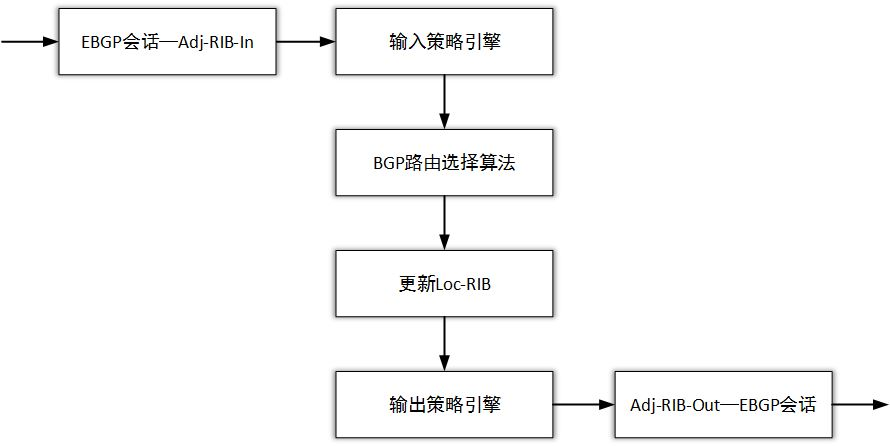
\includegraphics[width=\textwidth]{router}
  \caption{路由器的路由系统流程图\cite{journals/saem/KumarK14}}
  \label{fig:router}
\end{figure}

BGP协议运行在自治系统内的每台边界路由器上,每台边界路由器收到路由信息,会进行路由信息存储、应用路由策略、计算最优路由、更新本地路由表以及将路由进行出口过滤并转发等操作,其处理路由信息的流程如图\ref{fig:router}:所示,主要涉及三大模块:路由存储、路由策略、路由计算。

\subsection{路由存储}
运行BGP会话的边界路由器从其他对等体收到路由更新消息,其保留收到的信息,将信息进行处理生成最优路由用于本地数据包的转发,该边界路由器会基于预定义的策略向外宣告路由。在路由信息处理的过程中,路由信息存储在路由信息库(Routing Information Bases, RIBs)中,BGP的路由信息库\cite{rfc1771}中主要包含以下三张表:

\begin{itemize}
    \item Adj-RIBs-In:该表中存储了从不同对等体收到的未经路由入口过滤和属性修改的原始BGP路由信息,该信息用于BGP决策过程的输入。
    \item Local RIB:该表中存储了经过路由入口策略(过滤和BGP属性修改)的路由信息,此外该表中还使用selected标记了每一个前缀的最优路由。
    \item Adj-RIBs-Out:该表中存储了经过路由出口策略,即将被宣告给每一个对等体的最优路由信息。
\end{itemize}

\subsection{路由策略}
路由信息在自治系统间传输,每个自治系统如何影响路由选择和传递,需要依赖该自治系统部署的路由策略\cite{DianeTeare2016CCNP},可以过滤更新从邻居收到的路由信息,经过路由计算之后也可以过滤更新将宣告给邻居的路由信息。

路有更新过滤常见的4种工具\cite{Kocharians2015CCIE}:
\begin{itemize}
    \item 分布列表:通过配置访问列表对路由更新进行控制,配置路由器的网络管理员决定允许接收来自哪些IP的路由更新,拒绝接收哪些IP的路由更新。
    \item 前缀列表:针对从邻居收到或者转发给邻居的路由,应用前缀列表,对匹配上前缀列表正则表达式的前缀执行permit或者deny操作。
    \item AS-path访问列表:配置路由器的网络管理员根据eBGP路由中携带的AS-path属性内容,对路由信息进行过滤。
    \item route-map路由映射:路由映射在控制BGP更新方面非常灵活,可以匹配并设置多种不同的BGP属性。该操作分两部分:match匹配和set设置。如果路由匹配了一条route-map命令中的所有匹配项,说明该路由与之匹配,则执行路由映射命令中的设置(修改路由属性,permit或者deny)。
\end{itemize}


分布列表、前缀列表、AS-path访问列表、路由映射都可以用来入站出站路由的过滤更新,不同的路由设备中BGP过滤更新机制的执行顺序可能不同。本文研究实现基于Quagga\cite{quagga}软件路由器平台,Quagga的入站出站过滤更新顺序见下:

\begin{itemize}
\item Quagga入站过滤更新顺序:分布列表、前缀列表、AS-path访问列表、路由映射。
\item Quagga出站过滤更新顺序:前缀列表、分布列表、AS-path访问列表、路由映射。
\end{itemize}

\subsection{路由选择算法}
BGP路由计算\cite{DianeTeare2016CCNP}的过程是为了选择最优路由,BGP最优路由的选择是根据BGP属性执行的。同一个前缀可能有多条路由,BGP会选择一条最优路由,来传输去往这个前缀目的地址的流量,不同的路由设备路由计算的算法有微小差异,以Quagga软件路由器中BGP的实现为例,同一条前缀的多跳路由(不构成AS环路且下一跳有效可达),根据收到时间由近及远,两两比较,得到最优路由。比较的过程如下所示,不断执行以下步骤直到选出最优路由:

\begin{itemize}
    \item 步骤1:优选权重(Weight)最高的路由,Weight属性本地路由器有效。
    \item 步骤2:优选本地优先级(Local Preference)最高的路由,自治系统内有效。
    \item 步骤3:优选本地路由器初始的路由(本地初始的路由在BGP表中的下一跳显示为0.0.0.0)。
    \item 步骤4:优选as-path最短的路由。
    \item 步骤5:优选源代码(Origin code)最小的路由(IGP<EGP<不完整路由)。
    \item 步骤6:优选MED(Multi-Exit Discriminators,多出口鉴别符)最低的路径,只有当所有待选路由来自同一AS时,路由器才会对比MED。网络管理员也可以通过设置路由器配置命令bgp always-compare-med,使得MED值总是可比。
    \item 步骤7:优选外部eBGP路由,而不是内部iBGP路由。
    \item 步骤8:优选去往BGP下一跳最短的路径,即IGPcost最小的路由。
    \item 步骤9:优选eBGP最老的路由,减少路由反复启动和禁用的风险。
    \item 步骤10:优选邻居BGP路由器ID值router-id最低的路由。
    \item 步骤11:优选邻居IP地址最小的路由。
\end{itemize}

本小节介绍了BGP协议以其工作流程,熟悉BGP处理路由信息的流程有助于利用集中式的思路解决且优化iBGP存在的一些问题。

\section{iBGP协议存在的问题}

早期iBGP协议运行在某个自治系统内部的边界路由器上,因为iBGP连接中路由信息仅能传播一跳(域内的边界路由器收到iBGP邻居的路由信息,不能再将其进行转发传播),所以域内的iBGP路由器必须以全网状Full-mesh的结构相连,保证路由信息传输到每一台路由器,所以随着网络规模的不断扩大,自治系统内部的边界路由器逐渐增多,全网的路由越来越多(Potaroo\cite{bgptabledata}显示IPv4的路由表项约有70万条),路由更新越来越频繁(Potaroo显示路由表每秒最多更新2000条),网络拓扑连接和路由策略越来越复杂,iBGP协议面临很大的挑战\cite{ibgp2016infocom},比如糟糕的可扩展性、配置文件的负担越来越大、域内用于路由信息传输的BGP控制报文占用更多的带宽资源、路由表的冗余存储等等。现在,传统的Full-mesh模式的iBGP结构仅应用于规模比较小的自治系统内,规模比较大的自治系统一般使用比较容易部署的且不需要Full-mesh连接的路由反射\cite{rfc2796}模式。

iBGP\cite{Oprescu2011Rethinking}目前存在三方面问题:可扩展性差,域内路由决策非最优出口,复杂路由策略难以管理。

iBGP协议必须保持全连接,防止在AS内部形成BGP路由环路,同时确保BGP路由路径上的所有路由器将数据报正确地转发到目的地。全连接导致每台边界路由器需要和域内的其他边界路由器维护iBGP会话,整个域内的iBGP会话数量是边界路由器总数的平方数量级,同时随着BGP路由表加速增长对路由器的存储和计算能力提出了更高的要求,路由表的数量从2001年的约10万条已经增长到2018年的约70万条,iBGP的可扩展性问题日益显著。

自治系统内的边界路由器收到路由后,会通过iBGP连接将该路由对应前缀的最优路由,传输给相连的iBGP对等体。如果自治系统内部的iBGP连接是路由反射结构,路由反射器收到路由之后,会计算最优路由,将最优路由宣告给与该反射器在同一个集群的客户端。这直接导致了某些边界路由器没有收到全部路由。在路由计算的过程中,如果没有基于全部路由计算,或者仅考虑了IGP cost,没有考虑域内的拓扑等其他信息,这些均有可能导致自治系统内的每台边界路由器上的路由计算结果非最优出口。

自治系统的策略需要在自治系统内的每台边界路由器上进行配置,随着网络规模的不断扩大,网络中新功能新需求的不断增加,自治系统的策略越来越复杂(2018年Cernet2核心路由器的BGP配置文件已达5万行),复杂的路由策略需要配置在每一台边界路由器上,非常容易误配置,或者出现边界路由器策略配置不一致的现象。如果想要修改策略,则需要修改相对应的所有边界路由器上的配置,配置在每台边界路由器上的路由配置文件难以管理、难以更新。

随着网络规模和需求不断增长,路由表的规模和域间的BGP消息也越来越多,iBGP结构的可扩展性已经成为iBGP存在的最重要最有挑战性 的问题之一。

\begin{figure}
  \centering
  % Requires \usepackage{graphicx}
  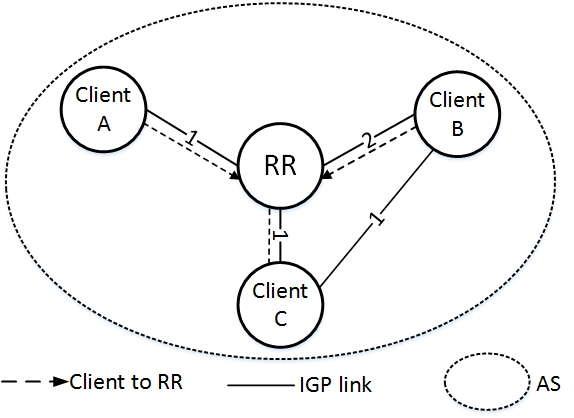
\includegraphics[width=\textwidth]{rr-nobest}
  \caption{路由反射引起的非最优出口举例\cite{Feamster2004The}}
  \label{fig:rr-nobest}
\end{figure}

\section{现有解决iBGP可扩展问题的相关研究}
现有解决iBGP可扩展问题的相关研究,根据体系结构思想和设计,大致可以分成两类:分布式路由体系结构下的相关研究(路由反射\cite{rfc2796}、AS联邦\cite{rfc1965})和集中式路由体系结构下的相关研究(SoftRouter\cite{lakshman2004}、RCP\cite{Feamster2004The}、RFCP\cite{Rothenberg})。分布式路由体系结构中所有的网络功能等均由路由器实现,传统网络使用的是分布式路由体系结构,数据平面和控制平面的功能都集中在同一个平台(路由器)上实现,数据平面和控制平面的任何变动均会影响网络路由协议。集中式路由体系结构\cite{centralization}将数据平面和控制平面进行分离,在集中平台上实现网络的控制功能,减少了路由器的功能需求。

\subsection{分布式路由体系结构下的相关研究}
传统的分布式体系结构:路由反射和AS联邦,解决了iBGP全连接引起的可扩展问题,但其设计本身可能导致选择路由不是最优出口、路由震荡、转发环路等问题。

\subsubsection{路由反射\cite{rfc2796}}

2000年,针对iBGP的可扩展问题,T.Bates等人在RFC2796\cite{rfc2796}中提出了路由反射。路由反射是将自治系统内的边界路由器分成多个集群,每个集群里面有一个或者多个路由反射器,集群中其他的路由器称之为客户机(Client)。客户机仅与自己的路由反射器RR建立iBGP连接,路由反射器之间建立Full-Mesh的iBGP连接。当RR收到一条路由更新:如果该路由从非client的iBGP对等体收到,RR将最优路由反射给所有的clients;如果该路由从client的iBGP对等体收到,RR将最优路由反射给其他的RR和所在cluster里面的clients。



路由反射因为缺少全部路由和结构设计等问题,在特定条件下会产生非最优出口、转发环路、路由震荡等问题。


路由反射导致的非最优出口问题根本原因是,路由反射器计算出来的最优路由并不是Client的最优路由,如图\ref{fig:rr-nobest},假设RR收到前缀Prefix1的路由信息,RR经过路由计算后发现Client-A为Prefix1的最优出口,RR会将Prefix1的最优出口为Client-A这条消息宣告给Client-B和Client-C,Client-C会认为Prefix1的最优出口为Client-A,实际上对于Client-C而言,Client-B为Prefix1的最优出口。

\begin{figure}
  \centering
  % Requires \usepackage{graphicx}
  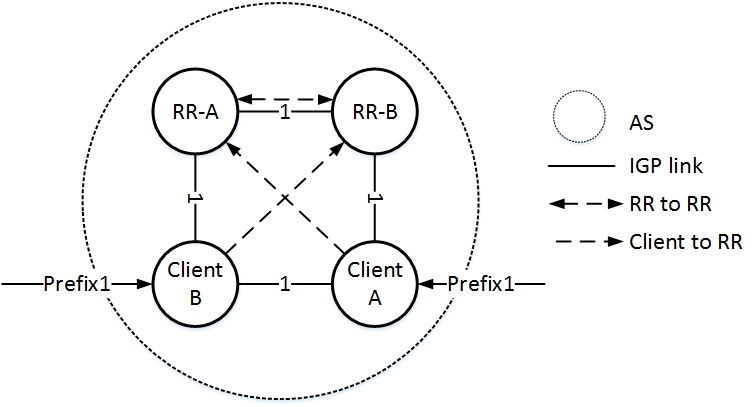
\includegraphics[width=\textwidth]{rr-forwardloop}
  \caption{路由反射引起的转发环路举例\cite{ibgp2016infocom}}
  \label{fig:rr-forwardloop}
\end{figure}



路由反射导致的转发环路根本原因是,路由反射结构设计不合理,物理链路和逻辑链路不一致,路由反射器最优出口的ospf路径经过了其他的路由反射器,该数据包被重新路由,如图\ref{fig:rr-forwardloop},形成转发环路的过程:

\begin{itemize}
\item 步骤1:Client-A和Client-B收到相同前缀Prefix1,分别通告给自己的反射器;
\item 步骤2:RR-A认为Prefix1的最优出口为Client-A;RR-B认为Prefix1的最优出口为Client-B;
\item 步骤3:RR-A收到目的地址为Prefix1的数据包,判断该数据包的最优出口为Client-A,根据IGP链路要到达client-A必须经过RR-B,所以RR-A将目的地址为Prefix1的数据包转发给RR-B。
\item 步骤4:RR-B收到目的地址为Prefix1的数据包,判断该数据包的最优出口为Client-B,根据IGP链路要到达Clinet-B必须经过RR-A。所以RR-B将目的地址为Prefix1的数据包转发给RR-A。
\item 步骤5:RR-A又转发给RR-B(步骤3),RR-B转发给RR-A(步骤4),形成了转发环路(步骤3和步骤4不断重复)。
\end{itemize}



路由反射导致的路由震荡有两种典型的情况:MED震荡(因为MED不可比产生的路由震荡)和拓扑震荡(因为RR拓扑设计不合理产生的路由震荡)。


\begin{figure}
  \centering
  % Requires \usepackage{graphicx}
  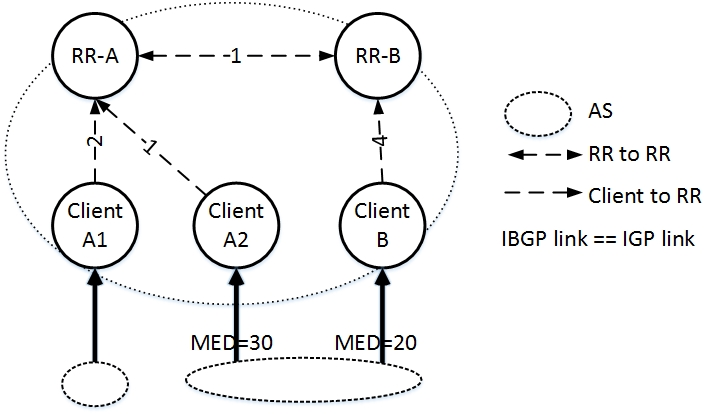
\includegraphics[width=\textwidth]{rr-med}
  \caption{路由反射引起的MED震荡举例\cite{Flavel2009Stable}}
  \label{fig:rr-med}
\end{figure}


路由反射因为MED震荡,根本原因在于路由计算的过程中某些度量值(MED)不可比,如图\ref{fig:rr-med},因为不同时刻路由反射器针对同一Prefix产生的最优路由不同,导致其他路由反射器在不同时候收到的同一Prefix的路由集不同以至于该Prefix的最优路由不同,形成的MED震荡过程如下:

注:传输到域内的3条路由,前缀、Weight、Local Preference、aspath均相同。

\begin{itemize}
\item 步骤1:RR-A从Client-A1和Client-A2收到前缀Prefix1的路由,先收到Client-A1,再收到Client-A2, 因为Client-A2到RR-A的IGPcost更小,所以RR-A收到2条Prefix1的路由,选择来自Client-A2的路由为Prefix1的最优路由;
\item 步骤2:RR-A将Prefix1的最优路由宣告给RR-B,RR-B收到来自Client-A2和Client-B的路由,因为Client-A2和Client-B收到的路由来自于同一个自治系统,所以MED值可以比较,最终RR-B选择来自MED值更小的Client-B过来的路由;
\item 步骤3:RR-B将Prefix1的最优路由宣告给RR-A,RR-A收到来自Client-B、Client-A2、Client-A1的总共3条路由,因为路由计算是把由近及远的路由两两比较,那么RR-A进行路由计算的时候先因为MED值可比淘汰掉来自Client-A2的路由,然后将Client-B和client-A2进行比较,因为MED值不可比取IGPcost更小的路由,则RR-A选择来自Client-A1的路由为Prefix1的最优路由;
\item 步骤4:RR-A将Prefix1的最优路由宣告给RR-B,则RR-B收到来自Client-A1和Client-B的路由,因为MED不可比取IGPcost更小的路由,则RR-B选择来自Client-A1的路由为Prefix1的最优路由;
\item 步骤5:RR-B将Prefix1的最优路由,宣告给RR-A,则RR-A处只有来自Client-A1和Client-A2的两条路由了,回到步骤1,发生路由震荡...
\end{itemize}


\begin{figure}
  \centering
  % Requires \usepackage{graphicx}
  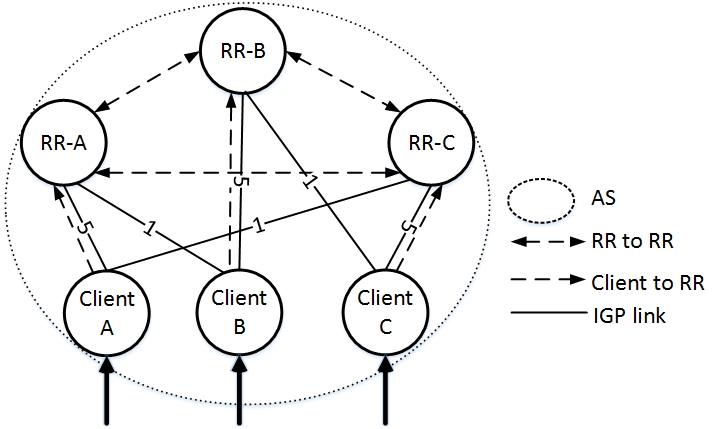
\includegraphics[width=\textwidth]{rr-topo}
  \caption{路由反射引起的拓扑震荡举例\cite{ibgp2016infocom}}
  \label{fig:rr-topo}
\end{figure}



路由反射导致的拓扑震荡,根本原因是RR结构设计不合理,cluster内部的RR和client之间的IGPcost远大于RR和其他cluster内的client的IGPcost,路由决策主要依赖IGP信息,如图\ref{fig:rr-topo},产生路由震荡的过程如下:

注:传输到域内的3条路由,前缀、Weight、Local Preference、aspath、MED均相同。

\begin{itemize}
\item 步骤1:RR-A收到来自Client-A的前缀为Prefix1的路由,RR-A只有1条路由,则选择来自Client-A的路由为Prefix1的最优路由,RR-A将Prefix1的来自Client-A的最优路由宣告给RR-B和RR-C;
\item 步骤2:RR-B有来自client-A、Client-B的2条路由,根据IGPcost选择来自Client-B的路由作为Prefix1的最优路由,RR-B会将Prefix1的来自Client-B的最优路由宣告给RR-A和RR-C;
\item 步骤3:RR-C有来自Client-A、Client-B、Client-C的3条路由,根据IGPcost选择来自Client-A的路由作为Prefix1的最优路由,RR-C会将Prefix1的来自Cleint-A的最优路由宣告给RR-A和RR-B;


\item 步骤4:RR-A有来自Client-A、Client-B的2条路由,根据IGPcost选择来自Client-B放入路由作为Prefix1的最优路由,RR-A将Prefix1的来自Client-B的最优路由宣告给RR-B和RR-C;
\item 步骤5:RR-B有来自Client-A、Client-B的2条路由,根据IGPcost选择来自Client-B的路由作为Prefix1的最优路由,RR-B会将Prefix1的来自Cleint-B的最优路由宣告给RR-A和RR-C;
\item 步骤6:RR-C有来自Client-B、Client-C的2条路由,根据IGPcost选择来自Client-C的路由作为Prefix1的最优路由,RR-C会将Prefix1的来自Client-C的最优路由宣告给RR-A和RR-B;


\item 步骤7:RR-A有来自Client-A、Client-B、Client-C的3条路由,根据IGPcost选择来自Client-B的路由作为Prefix1的最优路由,RR-A将Prefix1的来自Client-B的最优路由宣告给RR-B和RR-C;
\item 步骤8:RR-B有来自Client-B、Client-C的2条路由,根据IGPcost选择来自Client-C的路由作为Prefix1的最优路由,RR-B会将Prefix1的来自Cleint-C的最优路由宣告给RR-A和RR-C;
\item 步骤9:RR-C有来自Client-B、Client-C的2条路由,根据IGPcost选择来自Cleint-C的路由作为Prefix的最优路由,RR-C将Prefix1的来自Client-C的最优路由宣告给RR-A和RR-B;


\item 步骤10:RR-A有来自Client-A、Client-C的2条路由,根据IGPcost选择来自Client-A的路由作为Prefix1的最优路由,RR-A会将Prefix1的来自Cleint-A的最优路由宣告给RR-B和RR-C;
\item 步骤11:RR-B有来自client-A、Client-B、Client-C的3条路由,根据IGPcost选择来自Client-C的路由作为Prefix1的最优路由,RR-B会将Prefix1的来自Cleint-C的最优路由宣告给RR-A和RR-C;
\item 步骤12:RR-C有来自client-A、Client-C的2条路由,根据IGPcost选择来自Client-A的路由作为Prefix1的最优路由,RR-C会将Prefix1的来自Cleint-A的最优路由宣告给RR-A和RR-B;


\item 步骤13:RR-A有来自Client-A、Client-C的2条路由,根据IGPcost选择来自Client-A的路由作为Prefix1的最优路由,RR-A会将Prefix1的来自Cleint-A的最优路由宣告给RR-B和RR-C;(步骤1)
\item 步骤14:RR-B有来自client-A、Client-B的2条路由,根据IGPcost选择来自Client-B的路由作为Prefix1的最优路由,RR-B会将Prefix1的来自Cleint-B的最优路由宣告给RR-A和RR-C;(步骤2)
\item 步骤15:RR-C有来自Client-A、Client-B、Client-C的3条路由,根据IGPcost选择来自Client-A的路由作为Prefix1的最优路由,RR-C会将Prefix1的来自Cleint-A的最优路由宣告给RR-A和RR-B。(步骤3,开始循环发生路由震荡...)

\end{itemize}

\begin{figure}
  \centering
  % Requires \usepackage{graphicx}
  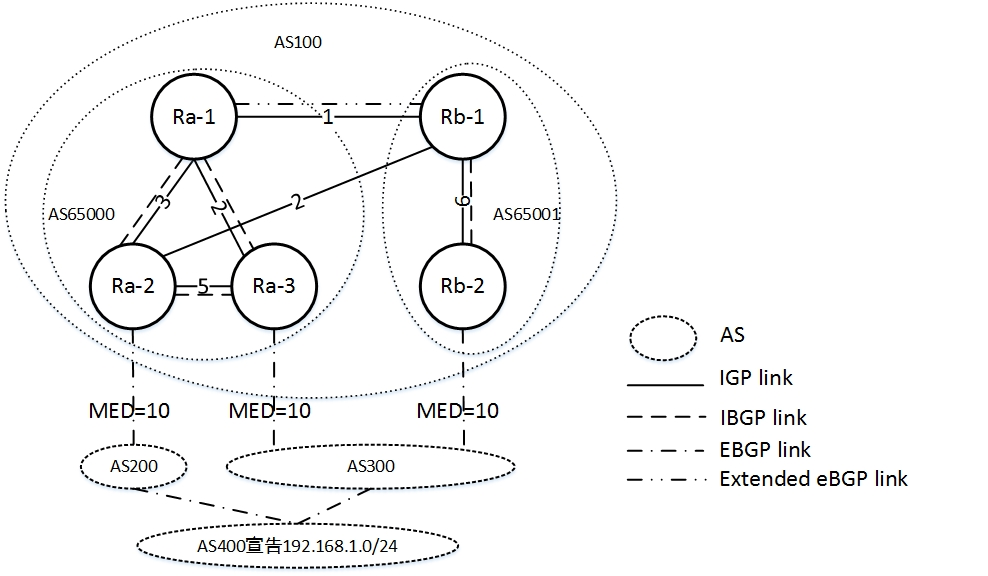
\includegraphics[width=\textwidth]{ascon-nobest}
  \caption{AS联邦引起的非最优出口举例}
  \label{fig:ascon-nobest}
\end{figure}


\subsubsection{AS联邦}


1996年,针对iBGP的可扩展问题,P.Traina等人在RFC1965\cite{rfc1965}中提出了AS联邦的方案。AS联邦的基本思想是将自治系统划分成多个子自治系统,子自治系统之间运行扩展的eBGP协议,子自治系统内部全连接,运行iBGP协议。

为了避免自治系统内出现路由信息环路,给自治系统内部的每一个子自治系统分配了Member-AS Number。当路由在域内传输的时候,通过检查经过子自治系统的Member-A Number序列,即可有效地防止域内路由信息传输的过程中发生环路。






AS联邦因为部分边界路由器在进行最优路由计算的时候,存在缺少全部路由和MED度量值不可比等问题,在特定条件下会产生最优路由计算结果非最优出口、路由震荡等问题。



AS联邦导致的非最优出口\cite{rfc5065},根本原因在于自治系统内部的子自治系统之间传输的是最优路由,那么子自治系统可能得不到全部的路由,该种情况下路由计算的结果则不一定是最优出口,如图\ref{fig:ascon-nobest},具体流程见下:

注:传输到域内的3条路由,前缀、Weight、Local Preference均相同。

\begin{itemize}
\item 步骤1:Ra-1收到来自Ra-2和Ra-3的路由Prefix1(前缀为192.168.1.0/24的路由信息),,Ra根据IGPcost最小原则选择来自Ra-3的路由作为Prefix1的最优路由,并宣告给Rb-1;
\item 步骤2:Rb-1收到Ra-1宣告的来自Ra-3的路由,Rb-1边界路由器有来自Ra-3和Rb-2的2条路由,根据IGPcost值最小Rb-1认为Prefix1的最优路由为来自Ra-3的路由。(实际对于Prefix1,Rb-1的最优出口是Ra-2,而不是Ra-3)
\end{itemize}


\begin{figure}
  \centering
  % Requires \usepackage{graphicx}
  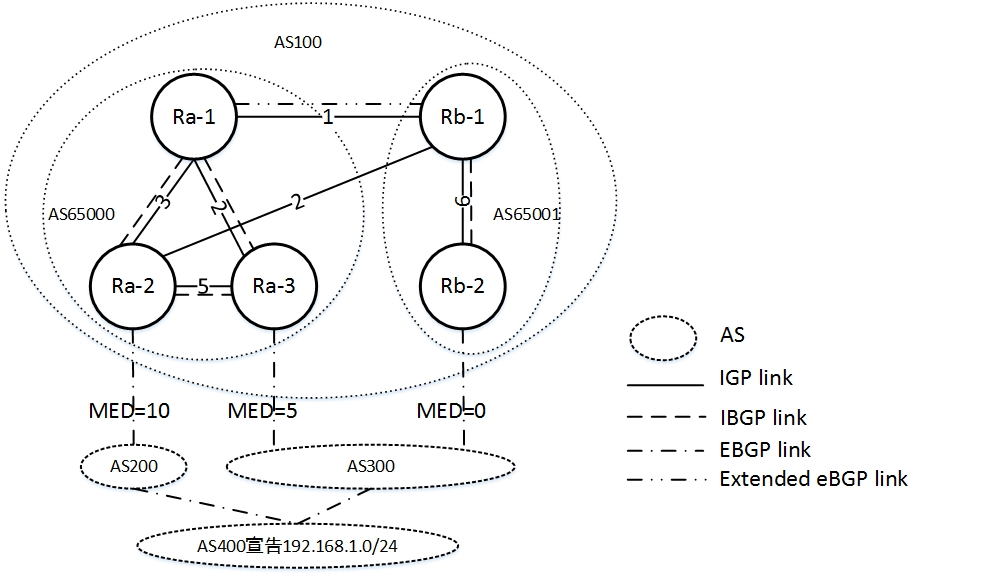
\includegraphics[width=\textwidth]{ascon-med}
  \caption{AS联邦引起的MED震荡举例}
  \label{fig:ascon-med}
\end{figure}

AS联邦导致的MED路由震荡\cite{rfc3345},根本原因在于路由计算的过程中没有基于全部的路由信息以及某些度量值(MED)不可比,如图\ref{fig:ascon-med},因为不同时刻子自治系统针对同一Prefix向外宣告的最优路由不同,导致其他子自治系统在不同时候收到的同一Prefix的路由集不同以至于计算出来的该Prefix的最优路由不同,形成的MED震荡过程如下:


\begin{itemize}
  \item 步骤1:Ra-1收到来自Ra-2和Ra-3的路由前缀为Prefix1(192.168.1.0/24的路由信息),,Ra根据IGPcost最小原则选择来自Ra-3的路由作为Prefix1的最优路由,并宣告给Rb-1;
  \item 步骤2:Rb-1收到Ra-1宣告的来自Ra-3的路由,Rb-1边界路由器有来自Ra-3和Rb-2的2条路由,根据MED值最小Rb-1认为Prefix1的最优路由为来自Rb-2的路由,并宣告给Ra-1;
  \item 步骤3:Ra-1有来自Rb-2、Ra-3、Ra-2的3条路由,由收到时间由近及远进行两两比较。先比较Rb-2和Ra-3,根据MED最小选择Rb-2。再将Rb-2和Ra-2一起比较,根据IGPcost最小选择来自Ra-2的路由作为Prefix1的最优路由,并宣告给Rb-1;
  \item 步骤4:Rb-1收到Ra-1宣告的来自Ra-2的路由,Rb-1边界路由器有来自Ra-2和Rb-2的2条路由,根据IGPcost值最小Rb-1认为Prefix1的最优路由为来自Ra-2的路由,并宣告给Ra-1;
  \item 回到步骤1,发生路由震荡。
\end{itemize}

\subsection{集中式路由体系结构下的相关研究}

集中式路由体系结构主要的思路是数据平面和控制平面分离。为了解决iBGP的可扩展问题,很多学者从集中式路由体系结构的思路切入,针对日益复杂的网络拓扑和管理控制功能,提出了一些具有代表性的工作,比如SoftRouter、RCP(Route Control Platform)、RFCP(Route Flow Control Platform),解决了iBGP的可扩展问题,同时也对路由存储、路由计算、策略部署等某个方面进行了优化。

\subsubsection{SoftRouter\cite{lakshman2004}}
SoftRouter的基本思想是将主控板(控制平面)从传统路由器中分离,配有主控板的路由器作为控制单元,配有线卡的路由器作为转发单元。转发单元和控制单元通过多对多的动态绑定进行连接,转发单元通过DDCP协议将自己绑定到最优的控制单元。控制单元之间通过iBGP协议进行Full-Mesh连接,转发单元和控制单元之间的信息交互通过ForCES\cite{rfc3746}协议,比如转发单元通过ForCES协议获得控制单元的转发表。

SoftRouter结构中,转发单元之间不需要建立Full-Mesh的全连接,这解决了iBGP可扩展问题。因为转发单元和控制单元已经完全分离,在控制单元上可以运行一些更复杂的安全协议。转发单元可以动态绑定到多个控制单元上,不同控制单元执行路由器不同的功能,所以SoftRouter也容易部署开发新的功能。此外,自治系统内的主控板的总数减少,运营商的开支也相对应地减少。

Softrouter也存在一定的局限性,列举其中主要的三点局限性:
\begin{itemize}
  \item 转发单元和控制单元多对多的连接结构,使得Softrouter整体的结构十分复杂,其本身的可扩展性非常差;
  \item 在路由计算的过程中,仍使用传统的主控板进行计算,并没有考虑IGP视图,导致路由计算的结构不够灵活;
  \item 转发单元上不同的功能策略在不同的控制单元上进行配置,不同控制单元部署下发的策略可能存在矛盾、覆盖等情况。
\end{itemize}

\begin{figure}
  \centering
  % Requires \usepackage{graphicx}
  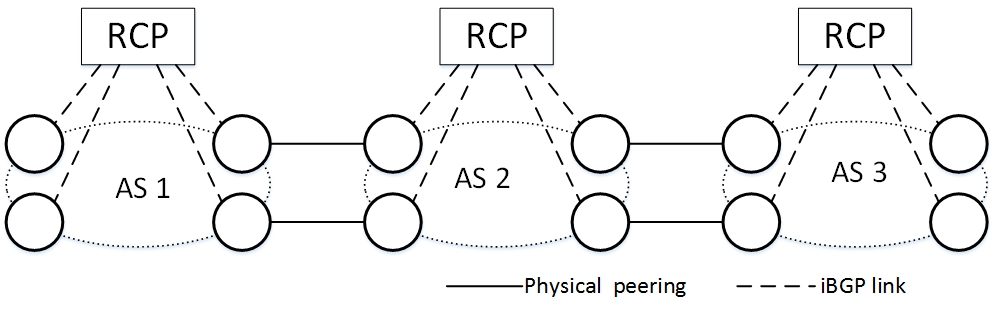
\includegraphics[width=\textwidth]{rcp}
  \caption{Routing Control Platform in the Internet\cite{Feamster2004The}}
  \label{fig:rcp}
\end{figure}

\subsubsection{RCP\cite{Feamster2004The}}
RCP(Route Control Platform,路由控制平台)的基本思想是在自治系统内部建立一个集中控制平台,通过与自治系统内的边界路由器建立iBGP连接来接收从eBGP连接传输过来的路由,在集中控制平台上进行集中式路由存储、策略应用和路由计算,最终得到自治系统内每台边界路由器的最优路由,通过iBGP下发到每台边界路由器,由边界路由器进行eBGP宣告。如果eBGP邻居的自治系统也部署了RCP平台,那么RCP平台之间可以直接建立Inter-AS协议连接进行通信,大概框架如图\ref{fig:rcp}。

基于RCP的思想,有学者提出了RCP的具体实现方案\cite{Caldwell2005Design},即在集中控制平台上运行三个模块,分别为BGP Engine,IGP Viewer和Route Control Server,BGP Engine负责和自治系统内的边界路由器通信,IGP Viewer负责即时收集域内拓扑信息,将对应的IGPcost矩阵传给Control Server,Control Server负责路由表的集中存储、路由策略的管理以及最优路由的计算等控制平面的功能。

RCP集中式控制平台可以进行集中式的路由存储,路由器上不需要存储路由表,极大地减少了路由器的负载。RCP集中式控制平台能够更好地进行策略管理,网络操作员在集中平台上部署路由策略,而不是专门去修改每台物理路由器上的路由配置文件。RCP集中式控制平台拥有集中的计算资源、整个自治系统内的IGP拓扑和传入自治系统的全部路由,能够更好地更准确地进行路由计算。

除了以上的优势,RCP也存在一些缺点\cite{Feamster2004The}:
\begin{itemize}
    \item 因为RCP平台本身既支持可能有上百条的iBGP连接,也支持可能上千条的eBGP连接,所以虽然解决了iBGP的可扩展问题,但是平台本身的可扩展性较差,集中平台需要针对每一条更新的路由,为域内的每一台边界路由器计算出该前缀对应的最优路由,可能集中平台的计算能力会受到很大的挑战;
    \item 集中平台都存在鲁棒性较差的特点,一旦集中控制平台的掌控控制单元的核心物理机器出现问题,整个自治系统的网络面临瘫痪的危险;
    \item RCP在策略集中配置的过程中,未考虑对集中的策略配置进行检测,预防策略冲突、覆盖等问题;
    \item RCP的路由计算仍属于传统的分布式路由计算,当收到一条更新路由时,需要计算N次得到N台路由器的最优出口路由。
\end{itemize}

\subsubsection{RFCP}
RFCP(Route Flow Control Platform,图11)是基于SDN的思想,集中式地收集信息,在APP运行多台虚拟机,模拟自治系统环境,分布式地计算路由,并通过SDN平台传递给真实自治系统内的边界路由器。

RFCP可以集中式地对数据进行管理,通过流表规则下发对数据包和路由信息包进行转发,但RFCP结构中路由表冗余存储、路由计算未考虑IGP拓扑且仍为分布式计算,路由策略通过南向接口将策略传给控制器,未集中配置。

\section{集中式思路优化BGP的相关研究}

\subsection{SDX}
SDX

\subsection{集中式路由计算}
路由计算

\subsection{SDN+ibgp}

SDN和BGPgggg\cite{conf/cfi/2014}


\section{本章小结}

综合以上的调研,RR、AS联邦、3种集中式体系结构的方案虽然解决了iBGP可扩展问题,但RR和AS联邦带来了新问题;3种集中式方案对路由存储、计算、策略管理的某些方面进行优化,具体的对比见图13。
本课题提出新结构,能够解决iBGP可扩展性,同时最大限度优化路由存储和计算、策略管理。路由表RIB仅存储在集中控制平台,路由计算在集中平台上计算,依赖自治系统内的网络拓扑信息,支持多输入多输出的计算模式,拟计算一次(最坏情况下计算N次)得出所有边界路由器针对Prefix的最优路由。
